%!TEX ROOT = thesis.tex
\chapter{Introduction}
\section{Basic Introduction}
%In the Introduction section, you should describe the problem investigated. Try to summarize relevant research to provide context, key terms, and concept so the reader can understand the whole final year project. Go and read journal or conference papers and review relevant past research to 
%provide rational or justification for your work. Define clearly your final project objectives and briefly describe your research – design, 
%research, hypothesis, etc.
Currently, the amount of vehicles on the road increases every year in Malaysia. It is because the local brand car is affordable by many low-income level household. The manufacturer also provided promotions to attract people to buy cars. As the result, the number of non-professional driver rapidly increased in Malaysia. Most of the drivers are unskilled and lack of awareness on the traffic safety and vehicle condition. The driver's personal factors have become the main reason of causing the traffic incidents.

According to the general road accident data in Malaysia taken from Malaysian Institute of Road Safety Research (MIROS) official website shown in Figure \ref{fig:accident}, the Malaysia government put effort on reducing the amount of traffic incidents by introducing the new traffic laws and speed tracking system. However, the number of cases of road deaths does not drop significantly.

\begin{figure}[hbt!]\centering
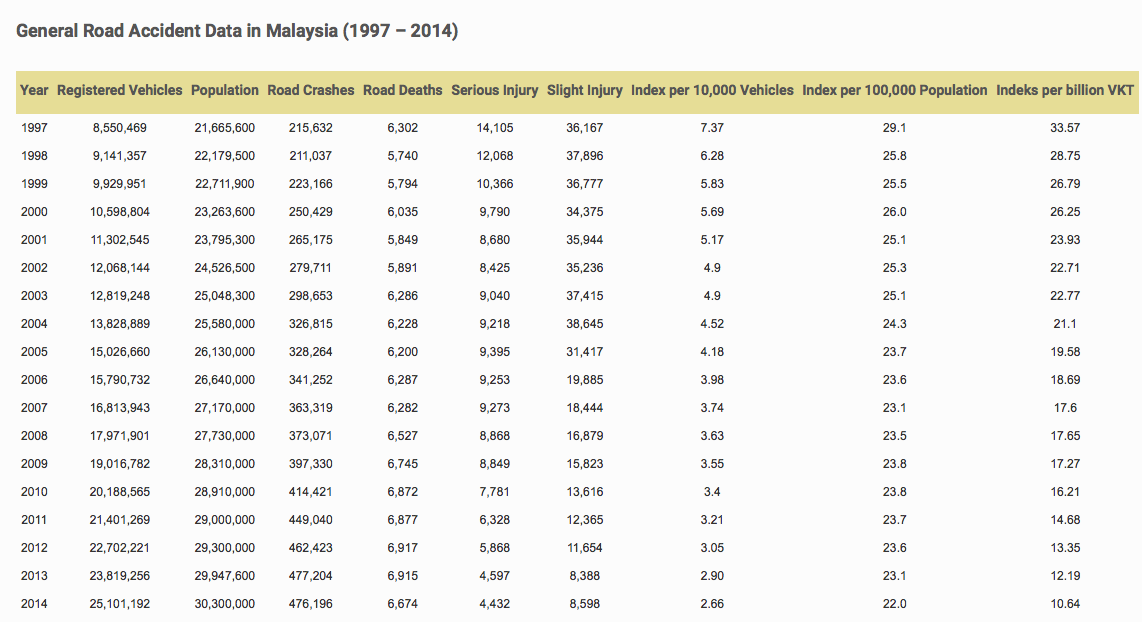
\includegraphics[width=.75\textwidth]{image/accident}
\caption{General Road Accident Data in Malaysia (1997 - 2014)}
\label{fig:accident}
\end{figure}

The driver characteristics and the occurrence of traffic incident is interrelated. To further reduce the number of accidents, the safety equipment of the vehicle needs to be improved as well as the road regulations, but also pay attention to driver behaviour. The behaviour of the driver is hard to be identified. The driver behaviour is affected by environment, vehicle condition and the mental or physical state. One of the ways to identify driver behaviour is using the vehicle telemetry data.

\section{Project Objective}
\begin{enumerate}
\item To identify the features that contribute to the accuracy of the classification of the driver behaviour analysis from the vehicle telemetry data.
\item To classify each vehicle telemetry records.
\item To profile the drivers based on the labelled vehicle telemetry data.
\end{enumerate}

\section{Research Motivation}
The price of the driver insurance plan is same among people. High risk driver and low risk driver pay the same price for the insurance. Logically, the high risk driver should pay more. However, driver behaviour is hard to be determine as good or bad. 

\section{Project Scope}
This project focuses on the driver driving behaviour profiling. Actual vehicle telemetry data are captured by using sensor. The vehicle telemetry data will be collected and preprocessed before analysing. Each driver is required to drive the car for at least 8 minutes to collect data. The data will be recorded every second. For each driver, there are at least 480 records in the dataset. K Means algorithm is implemented in this project to cluster the vehicle operation records. Each record will be labelled as good, medium or bad condition. Based on the labelled records, the drivers will be categorized to three classes. The classes are low risk, medium risk and high risk. 

\section{Project Plan}
Proper time and resource management is important to complete this project. Table \ref{tbl:gantt1} shows a brief description of the project timeline.

\begin{table}[h!]
\begin{tabular}{|l|c|c|c|c|c|c|c|c|c|c|c|}
\hline
Task \textbackslash Week & 2 & 3 & 4 & 5 & 6 & 7 & 8 & 9 & 10 & 11 & 12 \\

\hline
Data Acquisition &  \cellcolor[HTML]{000000} & \cellcolor[HTML]{000000} & \cellcolor[HTML]{000000} & \cellcolor[HTML]{000000} & \cellcolor[HTML]{000000} & & & & & & \\

\hline
Literature Review & & \cellcolor[HTML]{000000} & \cellcolor[HTML]{000000} & \cellcolor[HTML]{000000} & \cellcolor[HTML]{000000} & & & & & & \\

\hline
Data Analysis using KNIME & & & & & & \cellcolor[HTML]{000000} & \cellcolor[HTML]{000000} & \cellcolor[HTML]{000000} & & & \\

\hline
Driver Driving Behaviour Profiling & & & & & & & & \cellcolor[HTML]{000000} & \cellcolor[HTML]{000000} &  & \\

\hline
Analysing Experimental Result & & & & & & & & & \cellcolor[HTML]{000000} & \cellcolor[HTML]{000000} & \\

\hline
Documentation and Report & & & & & & & & & \cellcolor[HTML]{000000} & \cellcolor[HTML]{000000} & \cellcolor[HTML]{000000} \\

\hline
Report Submission & & & & & & & & & & & \cellcolor[HTML]{000000}\\

\hline
\end{tabular}
\label{tbl:gantt1}
\caption{Project timeline of Final Year Project I for Trimester 1 2016/2017}
\end{table}